\chapter{Experiments and Evaluation}
\section{Serverless Computing}
\subsection{Managed container services}
\subsubsection{Test task and System Description}
// This is just a draft
In this experiment we simulate the continues delivery process of a Spring Boot web application in the DevOps toolchain developed by us. From the experiments, we could verify our assumption in \ref{assumption}.
The continues delivery pipeline includes following steps:
\begin{enumerate}
    \item \textit{Pull from version control}: Pull the most recent change from Github repository
    \item \textit{Build}: Build the application with Gradle
    \item \textit{Test}: Automate testing with JUnit integrated in Gradle
    \item \textit{Artefact store}: Push the build artifacts to Artifactory
\end{enumerate}
\begin{figure}[h]
    \centering
    \begin{minipage}{0.45\textwidth}
        \centering
        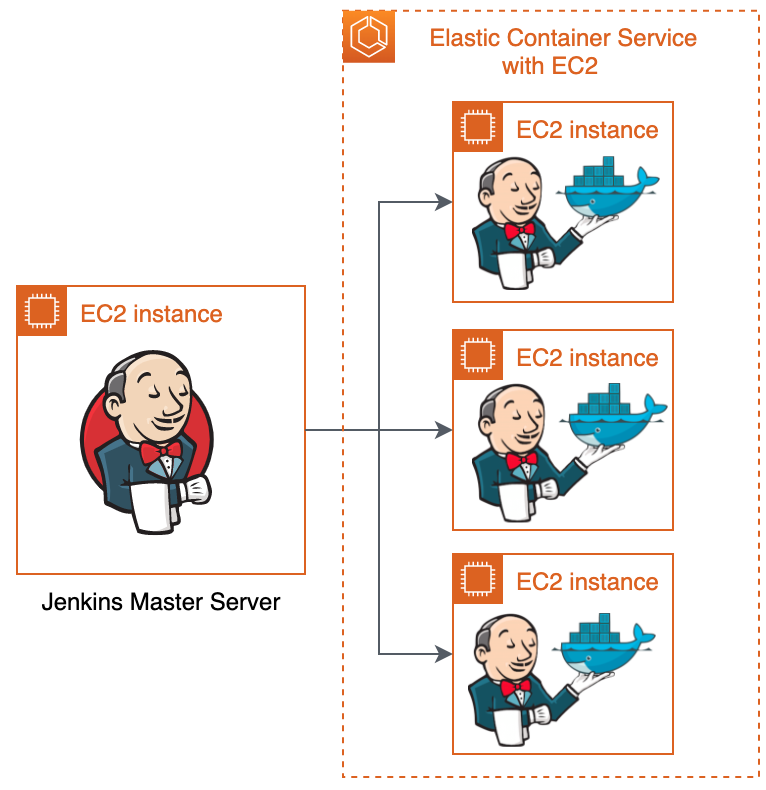
\includegraphics[width=\textwidth]{pics/jenkins-on-vm.png} % first figure itself
    \end{minipage}\hfill
    \begin{minipage}{0.54\textwidth}
        \centering
        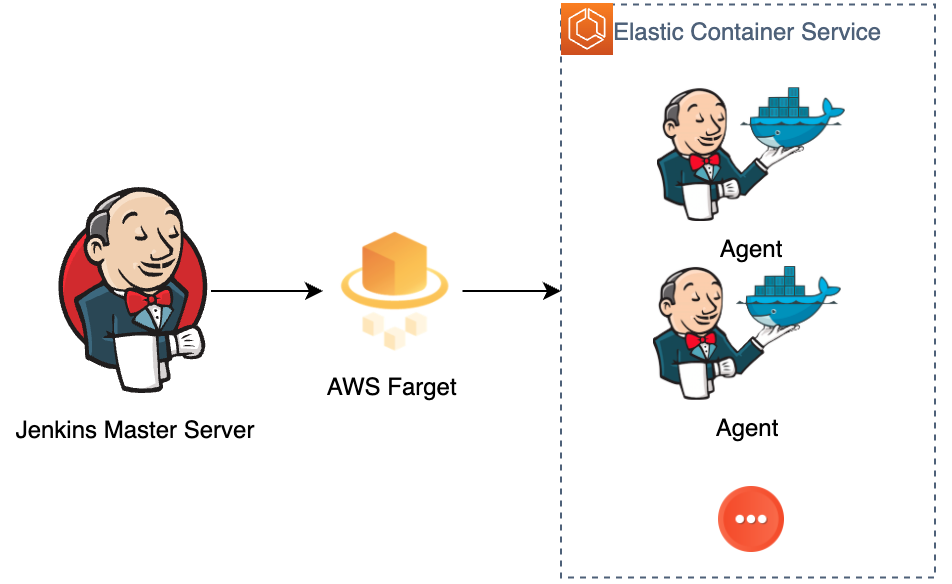
\includegraphics[width=\textwidth]{pics/jenkins-on-fargate.png} % second figure itself
    \end{minipage}
    \caption{Architecture diagram of the test Jenkins cluster with agents running in traditional virtual machine (left) and on ECS with AWS Fargate (right)}
\end{figure}
To evaluate our assumption in \ref{assumption}, we have 2 different setups. The first setup Figure 4.1 (left) is a Jenkins server with traditional virtual machine as worker agents. In the second setup Figure 4.1 (right), we use the same Jenkins server but the worker nodes is dynamically provisioned in the AWS Fargate managed cloud service.

// here write some more detail about the setup which includes IAM and hardware configuration, and also include the graph which shows the topological structure of 2 setups,

\subsubsection{Performance Properties and Evaluation}
We run the pipeline through 2 different setups, we will get the result of following properties:
\begin{itemize}
    \item \textit{Runtime} describes the total time for finishing all the tasks.
    \item \textit{Cost Structure} describes the daily cost of 2 setups under the same workload
    \item \textit{Resource Utilization} describes the average CPU/RAM usage for each instance during a single run of the pipeline.
\end{itemize}
To shows how does the 2 setups performance within the teams with different sizes, we run by run different number of tasks parallel through the pipeline. This simulates the different team size, besides, it could also shows the scalability when comes to the need of task parallelization in bigger organizations.
